\documentclass[class=article,crop=false]{standalone} \usepackage[margin=1in,headheight=57pt,headsep=0.1in]{geometry}
\usepackage[subpreambles=true]{standalone}
\usepackage{float}
\usepackage[framemethod=TikZ]{mdframed}
\usepackage{fancyhdr}
\usepackage[utf8]{inputenc} % Required for inputting international characters
\usepackage[T1]{fontenc} % Output font encoding for international characters
\usepackage{stix} % Use the STIX fonts
\usepackage{hyperref}
\hbadness=99999

\begin{document}
\subsection{Edit Item Form}
This is the form that is opened when you click the "Edit Item" (otherwise "Edit Element") button within the Edit Tile form, when the tile is of type "\texttt{item\_room}".
\begin{figure}[H]
	\centering
	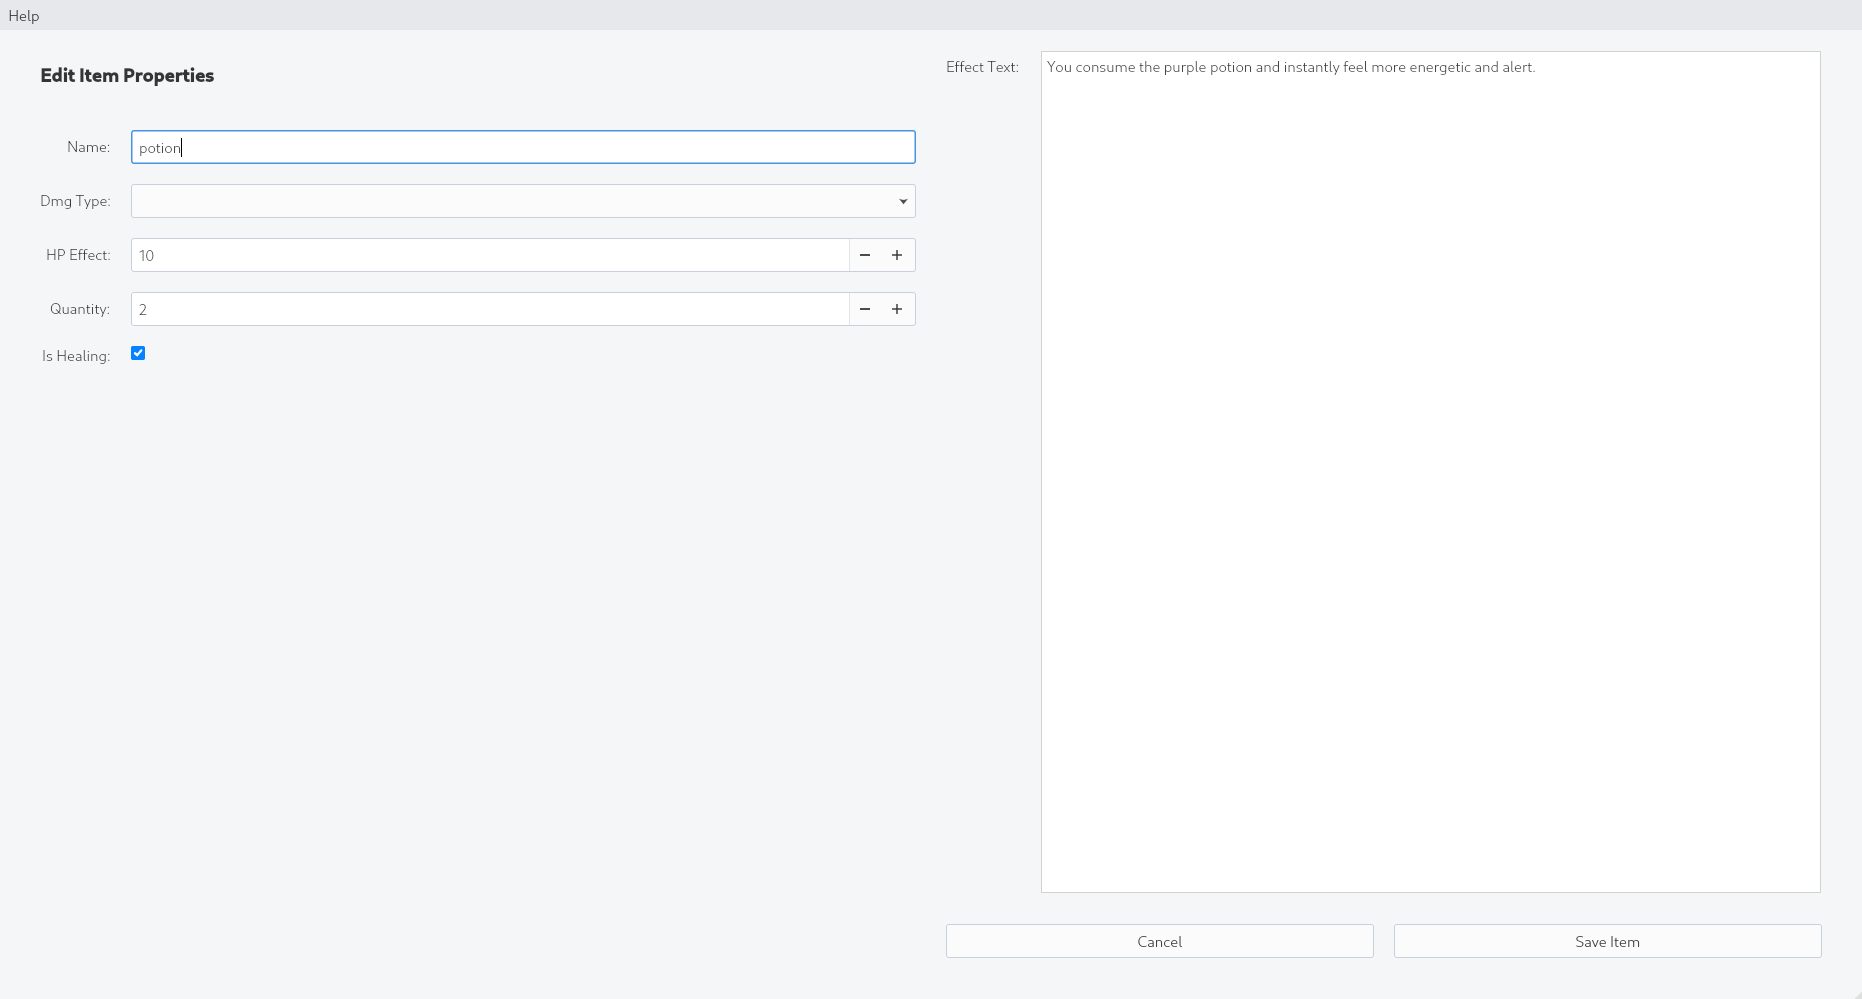
\includegraphics[width=1.0\textwidth]{./editItemForm.png}
\end{figure}
\begin{itemize}
	\item Name: this is the name of the item within the game, and it will be seen by the player.
	\item Dmg Type: the damage type of the item; in more complicated narratives this feature can be used to enrich gameplay. A weapon of a specific damage type interacting with an enemy of the same damage type deals potentially massive damamge.
	\item HP Effect: the maximum amount of damage inflicted by the item if it is a weapon, or the amount of player health the item heals if it is a consumable healing item. Note that the maximum player HP is 10.
	\item Quantity: the number of items contained in the tile overall. Note that an \texttt{item\_room} tile may only contain one type of item, but may possess multiple items of that type.
	\item "Is Healing" checkbox: Determines whether the item is a weapon that inflicts damage, or is a consumable healing item instead.
	\item Effect text: the text displayed to the player after consuming a the item, only relevant if "Is Healing" is checked.
	\item Cancel: closes the form without saving changes.
	\item Save Item: closes the form while saving the item to the parent Edit Tile form.
\end{itemize}
\end{document}
